% figS3_ensemble_hat.tex — TikZ v2 optimized
% Side-by-side: Standard HAT (single mask) vs Ensemble HAT (resampled masks)
\documentclass[tikz,border=10pt]{standalone}
\usepackage{amsmath}
\usepackage{amssymb}
\renewcommand{\familydefault}{\sfdefault}
\usepackage{tikz}
\usetikzlibrary{positioning,arrows.meta,shapes.geometric,fit,backgrounds,calc,decorations.pathreplacing,patterns,patterns.meta}

\definecolor{failRed}{RGB}{210,60,60}
\definecolor{failRedBg}{RGB}{255,225,225}
\definecolor{succGreen}{RGB}{40,160,70}
\definecolor{succGreenBg}{RGB}{215,245,225}
\definecolor{anaBlue}{RGB}{80,140,210}
\definecolor{maskColor}{RGB}{100,70,200}

\begin{document}
% Scale 0.95 for journal columnwidth compatibility
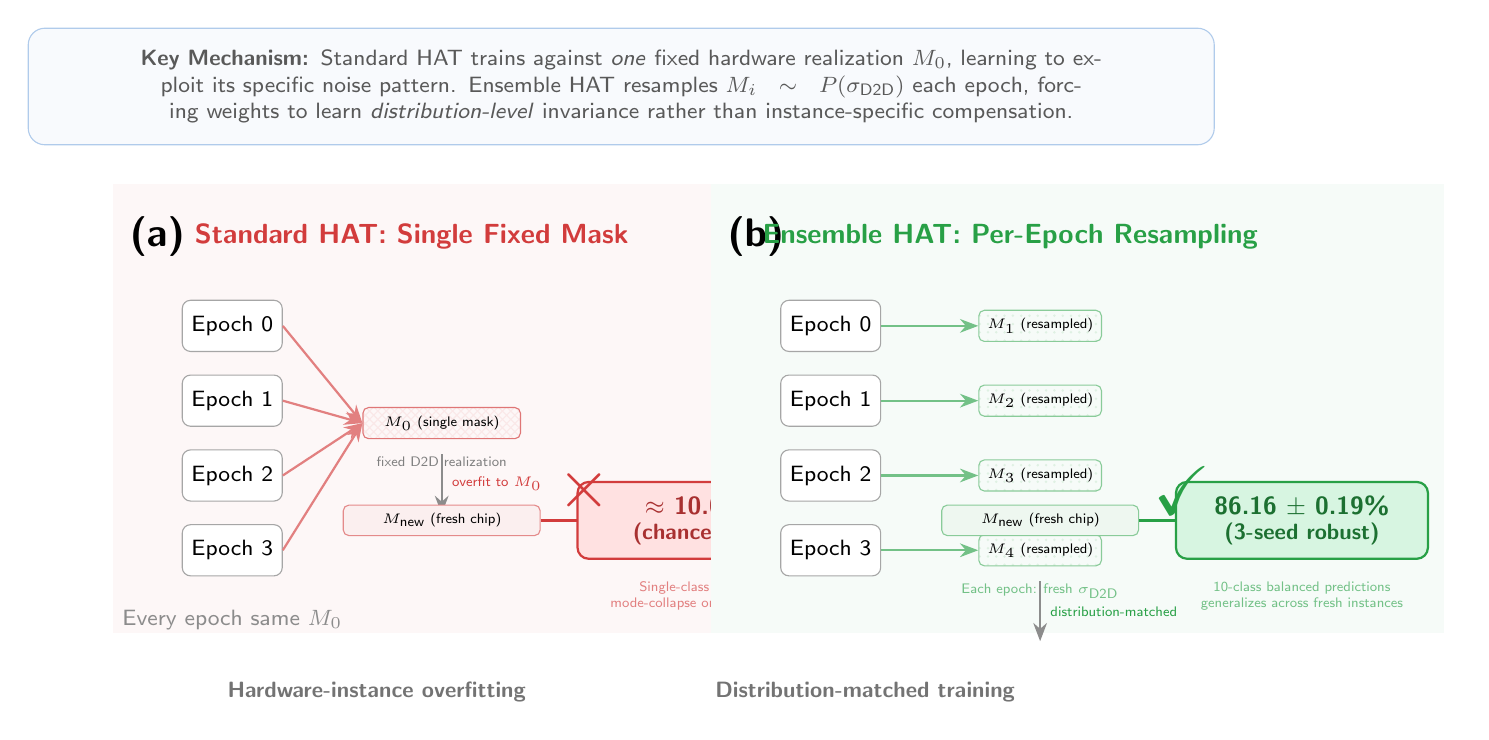
\begin{tikzpicture}[scale=0.95,
  epochbox/.style={draw=black!35, rounded corners=3pt, minimum width=1.1cm, minimum height=0.65cm, font=\footnotesize\sffamily, fill=white},
  maskbox/.style={draw=maskColor!65, rounded corners=2pt, fill=maskColor!4, font=\tiny\sffamily, inner sep=3pt},
  resultbox/.style={draw, rounded corners=4pt, thick, inner sep=5pt, font=\small\sffamily, minimum width=3.2cm, align=center},
  titlebox/.style={font=\bfseries\sffamily, align=center},
  arrowstyle/.style={->, >=Stealth, thick},
  panelmark/.style={font=\bfseries\sffamily\Large},
]

% ===================================================================
% PANEL (a) — Standard HAT (failure) with crosshatch
% ===================================================================
\begin{scope}[local bounding box=panelA]
  % Failure background shading
  \fill[failRed!4] (-2.8, 0.5) rectangle (7.0, 6.5);

  \node[panelmark] at (-2.2, 5.8) {(a)};
  \node[titlebox, text=failRed] at (1.2, 5.8) {Standard HAT: Single Fixed Mask};

  % Epochs
  \foreach \e in {0,1,2,3} {
    \node[epochbox] (E\e) at (-1.2, 4.6-\e*1.0) {Epoch \e};
  }

  % Single mask
  \node[maskbox, minimum width=2.0cm, pattern={crosshatch[distance=3pt]}, pattern color=failRed!12, draw=failRed!70] (M0) at (1.6, 3.3) {$M_0$ (single mask)};
  \node[font=\tiny\sffamily, text=black!50, below=0.1cm of M0] {fixed D2D realization};

  % Arrows epochs → mask
  \draw[arrowstyle, draw=failRed!65] (E0.east) -- (M0.west);
  \draw[arrowstyle, draw=failRed!65] (E1.east) -- (M0.west);
  \draw[arrowstyle, draw=failRed!65] (E2.east) -- (M0.west);
  \draw[arrowstyle, draw=failRed!65] (E3.east) -- (M0.west);

  \node[font=\footnotesize\sffamily, text=black!45, below=0.3cm of E3.south] {Every epoch same $M_0$};

  % Overfit arrow
  \draw[arrowstyle, draw=black!45, thick] ($(M0.south) + (0, -0.2)$) -- ++(0, -0.8)
    node[midway, right, font=\tiny\sffamily, text=failRed] {overfit to $M_0$};

  % Fresh instance
  \node[maskbox, minimum width=2.5cm, fill=failRed!8, draw=failRed!60] (MtestA) at (1.6, 2.0) {$M_{\text{new}}$ (fresh chip)};

  \draw[arrowstyle, draw=failRed, very thick] (MtestA.east) -- ++(1.5, 0)
    node[midway, above, font=\tiny\sffamily, text=failRed] {test};

  % Result
  \node[resultbox, fill=failRedBg, draw=failRed, font=\small\bfseries\sffamily, text=failRed!80!black] (ResA) at (5.1, 2.0)
    {$\approx$ 10.00\%\\[-2pt]{\footnotesize (chance level)}};

  \node[font=\tiny\sffamily, text=failRed!65, align=center, below=0.15cm of ResA.south, text width=3.8cm]
    {Single-class predictor\\ mode-collapse on fresh $\sigma_{\text{D2D}}$};

  % Red X
  \node[font=\Huge\sffamily, text=failRed] at (3.5, 2.4) {$\times$};
\end{scope}

% ===================================================================
% PANEL (b) — Ensemble HAT (success) with dots
% ===================================================================
\begin{scope}[shift={(8.0, 0)}, local bounding box=panelB]
  % Success background
  \fill[succGreen!4] (-2.8, 0.5) rectangle (7.0, 6.5);

  \node[panelmark] at (-2.2, 5.8) {(b)};
  \node[titlebox, text=succGreen] at (1.2, 5.8) {Ensemble HAT: Per-Epoch Resampling};

  % Epochs
  \foreach \e in {0,1,2,3} {
    \node[epochbox] (F\e) at (-1.2, 4.6-\e*1.0) {Epoch \e};
  }

  % Different masks per epoch
  \foreach \e in {0,1,2,3} {
    \pgfmathtruncatemacro{\midx}{\e+1}
    \pgfmathsetmacro{\my}{4.6-\e*1.0}
    \node[maskbox, fill=succGreen!6, draw=succGreen!55, pattern={dots[distance=2pt]}, pattern color=succGreen!15] (M\e) at (1.6, \my) {$M_{\midx}$ (resampled)};
    \draw[arrowstyle, draw=succGreen!65] (F\e.east) -- (M\e.west);
  }

  \node[font=\tiny\sffamily, text=succGreen!65, below=0.1cm of M3.south, align=center]
    {Each epoch: fresh $\sigma_{\text{D2D}}$};

  % Distribution-matched arrow
  \draw[arrowstyle, draw=black!45, thick] ($(M3.south) + (0, -0.2)$) -- ++(0, -0.8)
    node[midway, right, font=\tiny\sffamily, text=succGreen] {distribution-matched};

  % Fresh instance
  \node[maskbox, minimum width=2.5cm, fill=succGreen!8, draw=succGreen!55] (MtestB) at (1.6, 2.0) {$M_{\text{new}}$ (fresh chip)};

  \draw[arrowstyle, draw=succGreen, very thick] (MtestB.east) -- ++(1.5, 0)
    node[midway, above, font=\tiny\sffamily, text=succGreen] {test};

  % Result
  \node[resultbox, fill=succGreenBg, draw=succGreen, font=\small\bfseries\sffamily, text=succGreen!70!black] (ResB) at (5.1, 2.0)
    {86.16 $\pm$ 0.19\%\\[-2pt]{\footnotesize (3-seed robust)}};

  \node[font=\tiny\sffamily, text=succGreen!65, align=center, below=0.15cm of ResB.south, text width=3.8cm]
    {10-class balanced predictions\\ generalizes across fresh instances};

  % Green check
  \node[font=\Huge\sffamily, text=succGreen] at (3.5, 2.4) {$\checkmark$};
\end{scope}

% ===================================================================
% CENTER: Mechanism label
% ===================================================================
\node[font=\footnotesize\bfseries\sffamily, text=black!55, align=center] at (4.0, -0.3)
  {Hardware-instance overfitting \hspace{2.2cm} Distribution-matched training};

% ===================================================================
% TOP: Key insight box
% ===================================================================
\node[draw=anaBlue!45, rounded corners=6pt, fill=anaBlue!4, inner sep=8pt,
      font=\footnotesize\sffamily, text=black!65, align=center,
      text width=14.5cm] at (4.0, 7.8)
  {\textbf{Key Mechanism:} Standard HAT trains against \emph{one} fixed hardware realization $M_0$, learning to exploit its specific noise pattern.
   Ensemble HAT resamples $M_i \sim P(\sigma_{\text{D2D}})$ each epoch, forcing weights to learn \emph{distribution-level} invariance
   rather than instance-specific compensation.};

\end{tikzpicture}
\end{document}
